
    \section {物料计划与控制}

\subsection {物料控制过程}
.
    \begin{center}
        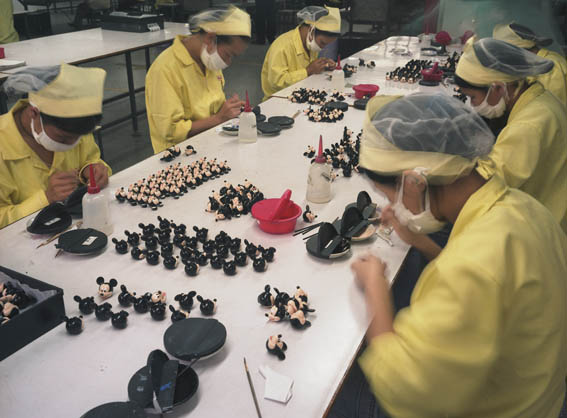
\includegraphics[scale=0.5]{pline1.jpg}
    \end{center}

    物料控制是为了控制好原料及其他物料的采购,不要出现近期生产不用却采购回大批物资积压在仓库,造成仓库库存太多,也不要出现马上该生产用原料了,而采购物资却仍不到位。最好是达到恰好要用恰好就到货,实现零库存或接近零库存的目的。

    物料控制的主要职能是物料计划、请购、物料调度、物料的控制(坏料控制和正常进出用料控制)等。物料控制通过制定行之有效的生产计划管理方案,使物料与生产管理工作顺畅,保证客户的需求,提高客户的满意度,同时提高生产效率,降低综合成本,进而提升公司的整体实力。

    对于接订单生产的企业。首先接到单后销售要把单传到物料控制员。并注明要求送货日期。物料控制员按排车间生产(有的是车间调度员安排,物料控制员只传单减库存)。按排生产的数量是单上要求到货数量加上动态库存数量减去仓库实际库存数量。生产部按照要生产的数量进行排程,并把排程结果交给物料控制员。物料控制员再计算该订单是否需要采购物料。采购物料到货日期就是生产订单前一天。

    物料控制的管理过程如下:

    职责分配:
        \begin{enumerate}
            \item  物料控制员对物料分析,使公司即不出现物料积压占压资金,又不出现停工待料。
            \item  市场部:负责订单下达及交期评审。
            \item  研发部:负责订单BOM制订及生产工艺设计。
            \item  PMC部:负责生产与物料计划的制订及协调跟进。
                \begin{enumerate}
                    \item  计划处:订单物料的发放、申购、跟踪及生产进度的跟踪。
                    \item  采购:负责物料的采购及跟进工作以及供应商评审。
                    \item  外发:负责物料的外发及进度跟进工作。
                    \item  货仓:负责物料进出仓控制及库存物料的质量控制。
                \end{enumerate}
            \item  生产部:负责生产前期准备工作及按计划完成生产任务,对生产进度及异常进行处理控制并反馈!
        \end{enumerate}

     \begin{enumerate}
        \item  交期评审:接订单后,市场部、研发部同PMC、生产部联合进行评审产品设计要求,货期,物料采购周期等,并出其《订单评审报告》。

        \item  编制生产计划:按评审的订单及时制订生产计划,包括生产进度计划,物料需求计划和设备要求计划。

            \begin{itemize}
                \item  生产计划
                    \begin{enumerate}
                        \item  对工厂设备人员,及生产能力进行分析评估,及香港上料之物料交期确认来制定具体生产计划。
                        \item  编制周生产计划,收集、汇总、縂计分析每日生产报表,根据生产进度异常,物料,技术,品质,工艺的变化,做生产计划调整。
                        \item  对生产进度落后,结合生产实际情况,同市场部沟通实际交期客人是否同意,再修正出货计划.
                    \end{enumerate}
                \item  物料控制:
                    \begin{enumerate}
                        \item  分解物料清单,根据仓库库存状况确定物料净需求量,根据经济订购量和生产计划,确定物料每次订购数量同交货期限,编制物料需求计划及订货计划。
                        \item  根据生产计划确认具体物料入库时间,协调采购,对可能缺料的订单重点跟踪处理因物料供应脱节、进度落后、生产提前、计划变更、订单变更而出现的物料问题。
                        \item  物料入仓后,开具《物料发放单》、生产据单到仓领料,物料发放应遵循先进先出,按单办理的原则。
                        \item  欠料和追料:根据每周的生产进度安排确认下周的物料缺料状况,对物料不能按期回厂和欠料情况,及时通知相关负责人跟进解决。并每3小时跟催一次,对物料不能回厂并影响生产的及时通知上司寻求共同解决.
                        \item  退料和补料:对生产所退仓物料进行分类标识并申请处理,对物料异常所产生的补料必须经上级签字后方能补数并留补料单备查。
                    \end{enumerate}
            \end{itemize}
        \item  货仓根据物料需求计划,查实仓储情况并及时反映给采购、计划、外发同时通知QC检查品质。
        \item  采购部根据物料需求计划订购所需物料并及时跟进物料回厂进度,做到适时供应生产物料。
        \item  外发根据物料需求计划同设备要求计划结合本厂实际情况时外发及跟进物料回厂进度。
        \item  生产根据生产进度计划进行编制作业组织生产,对各工序进度控制,异常调整,按时完成生产任务,成品经QA检验合格后填写,《成品入库单》,同仓库进行成品交接.
        \item  计划处出具出货计划表,合理间次安排装柜时间并通知香港船务部,仓库根据此安排入库工作并据香港船务部《收货通知单》安排装柜进行出库作业。
        \item  PMC每周出其货表共享,仓库及时填写《查货资料报告》并总结每月出货洭总。
    \end{enumerate}


\subsection {物料控制员}

    对制造业来说,实现ERP的计划与控制已大势所趋。然而,在企业管理人员当中,有一类人不仅压力最大,而且也充满了困惑。在新的变革到来时,尤其是传统的行业,企业的物料控制员要么是恐惧,要么是不知所措,为了不被信息时代所淘汰,他们孜孜不倦的求索:在信息化时代,我们应如何面对?

    物料需求计划的技法能产生一个实时的信息系统

    虽然物料需求计划MRP的技法能给我们带来一个实时的信息系统,并且产生恰当的信息,从而使物料控制员对信息采取行动。MRP的技法体现在如下几个方面。

    \begin{enumerate}
        \item  始终保持动态的供需平衡,是库存降低为最低点,而不缺料
        \item  可以自动的计算(现有库存+在订量+在检量-已分配量)
        \item  采购计划与生产计划自动算出,减少数据重复录入,减少人为的计算错误
        \item  主计划与生产计划与采购计划有效衔接
        \item  计划可重排性
        \item  计划可以反查
        \item  可以计算能力并能力分析
        \item  计划可以模拟
        \item  计划更实时,真实
        \item  对销售计划快速响应,提高准时发运率
        \item  提高团队精神(MRP牵涉到技术,库存,销售,生产等部门)
    \end{enumerate}

    那么,我们还需做什么呢?

\subsubsection {有效的物料控制员应该有一套工作程序来使工厂避免陷入困境。}

    一名成功的,有效的物料控制员应该提前告诉工厂经理即将来临的问题并推荐行动防止它们对客户服务或对工厂高效作业产生严重干扰。计划与控制的真正职能是为了使工厂避免陷入困境,从而管理工厂所需的信息而不只是处理为摆脱困境而要进行的日常活动。MRPII制造控制系统是一门处理信息的系统 ,它要求特定的活动要在特定的时间进行。 物料控制员像其它职能经理一样最好制订一张日程表把每天要求他们注意的事情列入表中并遵循这张表首先去做最重要的工作。没有一名经理能够去关心所有存在的问题,所以把问题排序并首先处理更重要的问题是极其重要的。

    由于物料控制员的成就将主要地依赖于信息系统的准确性与敏捷性,时常,某些最重要但是例行的活动(复审物料计划或提前期)是因为紧急中断的压力而被拖延的。有时要把后来表明的不良结果同其真正原因相联系是困难的。如列出一个检查清单会对正确地组织生产控制部门的活动有很大的帮助。物料控制员应该是定期地(至少每月一次)坐下来对下六个月里已知的与预期的问题作ABC分析,排出最大的问题并确保设计出活动来处理与防止这些问题。一个良好的习惯是每天准备一张今日按优先次序的活动表。

    物料控制员的工作计划(仅供参考)

    \begin{enumerate}
        \item  日程计划准备好
        \item  公布生产计划
        \item  修订生产计划
        \item  复审MRP输出表
        \item  查询缺货表
        \item  更新发出原料库存报告
        \item  完成"ABC"类存货复审
        \item  审计成品库存
        \item  活动与问题汇总
        \item  编制生产延误报告
        \item  编制外购组件延误报告
        \item  复审提前期
    \end{enumerate}

\subsubsection {物料控制员应主动的介入管理信息系统并成为协调者}

    计划与控制的主要职能是管理好一个信息系统。但是,必须强调的不是被动地去做。物料控制员在向管理层提出替代方案和这些方案的成本与结果的分析时应采取主动。在一个季节性销售的公司里,物料控制员应提出多种替代的生产计划以揭示如果完全用平准化生产,将额外地持有多少库存,如果按销售订单生产则将增加多大能力,人员将会有多少改变等等。物料控制员应估计这些不同计划的成本,推荐一份计划给管理层并协助做出基本的决策。一旦做出决策之后,物料控制员的工作就是控制信息使工厂保持在正常的轨道上。由于在过程中有许多计划的偏离,这就需要有不断的校正行动。 具有讽刺意味的是,生产线人员如果没有采取恰当的校正行动时,一个制造控制系统就难以被认为是成功的。实际上,仅仅产生了正确信息,这只是告诉经理们需要做什么而已。并不保证将采取的行动是正确的。往往物料控制员最容易受责难的原因是用其他人的行动来判断他的绩效。即使该系统指出需要增加能力而且这一增大能力的估计已经及早地通知了工厂作业人员或更高一级经理,但他们拖延不去增加,当结果使客户服务变差时,受埋怨的往往是计划与控制小组或物料控制员。几乎每个人都知道客户服务不好,但很少有人能识别出其真正原因。在ERP的管理信息运行的同时,物料控制员们经过有效的培训应该能采取行动。如果他们内行地做他们的处理信息的工作,他们将使所有有关人员知道需要采取什么行动并且谁要负责去采取这些行动。

    制造控制系统所生成的信息往往把巨大的压力施加在物料控制员的肩上,甚至加在往往是物料控制员上司的制造经理肩上。如果物料控制员对系统没有信心,如果他们不采取主动并且强有力地与勇敢地提出问题,他们会成为代人受过的“好人”,因别人不能采取恰当行动而自己受埋怨。制造控制系统必须能经得起来自物料控制员们的相当大的压力与挑战,他们总是对该系统产生的信息表示怀疑并要求作彻底的复审或进一步分析导致来推迟采取行动。能被证实的或能被容忍的怀疑态度的重要性应该有一个限度。在这一点上,能干的物料控制员应该得到其上司的强有利的支持以克服消极的阻力并采取有效的行动而不再进一步要求该系统证明它自己是可靠的。保持主动和进取心,再配上良好的系统与胜任的操作人员。每天,物料控制员们及其办事人员必须做出关于未来的成百甚至上千个决定。事后看来不可避免有些决定是错的,批评者很容易指出在计划过程中所犯的错误。所以物料控制员必须与其他经理们协调其工作目标为整个企业的目标。以避免在强调责任制的组织里会出现部门壁垒和信息孤岛现象。 物料控制员应承认救火是必要的,但防火才是更重要的。

    救火是必要的,但防火才是更重要的。制造控制中最严重的引诱之一就是去当一名救火员:每天早上一上班就准备接电话,然后马上冲出去。这毫无疑问地满足着那些强调行动的人,给人觉得非常有能力和可以把手指按在工厂脉搏上并随时知道什么事情正在进行中的经理的形象。不幸的是,这种救火活动在现实中是经常发生,但也是不可缺少的。导致防火的意识容易被忽视。如找出主要机床的寿命,弄清它们是否及时更新以达到所需能力或分析建议是否添置新产品的设备。何时,何处可能发生瓶颈,如何避免它们,这些工作看来确实是平凡的而不像救火一样轰轰烈烈。 忽视防火的物料控制员可以肯定明天将带来更大更好的救火机会。物料控制员必须对麻烦有思想准备。墨菲定律是“可能出错的问题,往往就在最不适宜的时间出现”就是在工厂里发明的。物料控制员应该是快乐的悲观者,他承认问题是一种生活方式,明天的问题今天毫无疑问正在酝酿着。工厂里的危机很少是一夜之间造成的,它们通常在一个长时期的酝酿而且时常是久久未采取行动的结果。物料控制员有责任及早指出麻烦可能出现何处,指出有哪些办法并做一切可能做的事去确保作业按计划持续进行或被校正以防止出现危机。 物料控制员必须在及时采取行动和未来准备改善计划之间取得平衡

    有效的控制信息的最主要特征之一就是它的及时性。是事后给出辩解还是及早地提出信息使得有人能采取措施去防止问题。如果物料控制员的上司询问为什么一种产品缺货了,而经过一些调查,他被告知它是由上周电镀部门一个瓶颈引起的,该物料控制员只是给出了一种辩解。如果,另一方面,该物料控制员早就曾指出该瓶颈并提出正面建议去克服它而且预言如果这个瓶颈不解决产品将会缺货,那么他就是发出了一个控制信息。这简单的差别就在于及时性,向工厂作业人员及时提供信息使他们在麻烦发生之前去采取必要的校正行动。

    为保持有效的运作,物料控制员必须用客观的,建设性的方式去使用他们的信息与知识的力量。他们应该是现实主义者,并避免乐观主义的痴心妄想,去指望麻烦可能不会发生或如果你不理它它就会自己跑掉。他们必需经常在提醒人们注意现存的与潜在的问题,可是,他们必须避免责备或说别人不能胜任并且不要忍不住去证明自己永远是正确的。

    物料控制员每天应抽出一些时间去访问工厂里主要的或关键的生产区域。往往快速地在工厂里兜一趟将发现潜在的问题比最最及时更新的信息系统还快得多。物料经理还必须抽出一点时间,这多半需要在工厂正规上班时间以外,去思考与计划对本部门未来绩效至关重要的事。这是他想出防火项目与改善本部门绩效的长期计划的时候。一名优秀的物料控制员应努力使解决今天问题的行动与防止明天问题的计划之间达到平衡。虽然其办公室的力量在解决许多日常危机中是需要的,但他们必须避免过多地直接介入于催稽之中。必须有一个为未来做准备的计划去平衡这种工作。

\subsubsection {物料控制员必须接受计划控制的教育与培训}

    为未来做准备最重要步骤之一就是培训。必须包括新技法、新系统、更现代化的设备的开发与使用的教育,以及通过参与专业机构去扩大眼界与听专门的课程以获得制造控制领域或其他企业管理领域的知识。这个教育还应包括厂内计划。我们大部分的生产管理人员开始从事计划与控制工作时并未在此领域中学习过。他们不仅对生产控制知识知之不多,而且往往并不理解有许多东西要学。这类人往往变成催稽员与救火人员而并无多大能力去有效地控制生产。实际上,现在该领域已成为具有独特知识主体、术语、技法与应用的一门真正的专业。目前,在国内,还没有一个专门的机构来认证合格的专业人员。如在财务领域,我们已有CPA资格考试,等等。而在国外,可以通过APICS参加考试,由此可被证明作为技术上合格的专业人员。

    目前,国内ERP培训,和各个软件功能培训比比皆是,而缺少像APICS这种机构,对专门从事生产控制人员的资格培训。我们在大力推广信息化的同时,往往忽视了基础的工作。 实际上,这种教育由于其对象主要是成年人,所以,尽可能切合实际。如果人们能具体地看到每种技法如何应用到他们的公司,或看到曾经在过去引起过的问题,他们会热烈地做出响应。每个人都有希望对自己的工作更加精通。然而,需要接受有关制造控制活动的教育培训的人远远超过计划与控制人员。公司里其它部门经常把计划控制小组当作替罪羊,对所产生的任何信息表示怀疑从而减少他们根据这一信息采取行动的需要。让这些部门主管懂得一个制造控制系统是什么,他们必须如何同它合作并使用它,他们提供的信息与他们所采取的行动会如何对系统的绩效产生影响,这是任何公司的成功所不可缺少的。 最高层管理人员往往对制造控制系统的真正作用也知之不多。他们不知道在库存与生产管理方面有效的替代方案是有限的而且并不总是意识到有必要去平衡日常作业中互相冲突的目标。一项广泛的教育培训计划,最起码可以让一部分人认识到从计划与控制活动可以期望什么与不可以期望什么。

    归根到底,一个乐于冒险去设定有雄心的目标的物料控制员,一个努力工作去改善部门的作业并在实施MRP生产与库存控制的经理、一个想提高客户服务水平,改善工厂整体绩效的经理,将不难说服管理层相信他的工作的重要性与价值。

\subsubsection {物料控制员必须降低库存}

    库存过多且伴以许多缺货已成为常规而非例外。而且可能还会持续一段时间,导致库存的原因有:

    \begin{enumerate}
        \item  不准确的预测与不可靠的供应,要求成品超过预期的需求。
        \item  不可靠的供应商与长而不确定的采购时间,使得过量的原料与外购组件成为必要。
        \item  经常的调整,不稳定的物流,不良的质量,报废与返工,不完善的机床安装与设备,使得大量的在制品成为必要。
        \item  种种变化引起报废的库存。
    \end{enumerate}

    现代的方法拒绝接受这些作为不可避免的条件。干扰计划作业的一切问题可以而且必须解决。管理层不断施加压力去减少库存是对的。事实证明,在任何公司里“正确的”库存量比现存于许多企业中的要少而比现存于大多数企业中的要少得多。正当的步骤如下:
    \begin{enumerate}
        \item  设定一个要在规定期间(例如6个月内)减少(譬如25%)的挑战性目标。
        \item  提出投入(外购物料与生产工时)与产出(发货)速率指标并每月监控它们。迅速而敢做敢为地去校正偏差。
        \item  使减少库存的目标成为公司范围的计划,各个部门都有角色要担当。只有通过找出并解决过剩的原因才能显著地削减库存。
    \end{enumerate}

\subsubsection {物料控制员必须缩短提前期}

    没有比缩短越提前期更重要的工作了。这种观点同制造作业中许多人所持的观点相反;他们都需要更多时间来确保更好的绩效。他们的经验通常支持这种信念:缺货需更长时间去克服,过多的负荷要用更多时间去处理,而延误是时间不够的证明。

    实际上,削减提前期已被证明是可能的,较容易的而且最为有效的。一项有效的措施是:

    \begin{enumerate}
        \item  用厂外与厂内课程进行教育培训
        \item  选择一个具有长而不稳定的提前期并供应着大量产品的供应商
        \item  选择具有大量订单积压的工作中心
        \item  选择不稳定负荷与太多的在制品的工序
        \item  设计更短的调整或换装
        \item  实施投入/产出控制
        \item  使物料保持流动,缩小批量
        \item  顶住非难,坚持信念
    \end{enumerate}

\subsubsection {生产计划与控制的未来}

    制造控制原先是一种文书工作职能:维护库存与订单记录,发放车间订单与处理其它必要的记录保管职能。从那里它发展到包括存货催促与一些部门的机器负荷计划──但大多数技法是粗糙的而功能高度分散,直到许多公司把库存控制从生产控制分离出来。导致每个小组倾向去考虑它自身的有限目标而不是公司的总体目标。这一朝着分散化的倾向使控制问题复杂化,因为它使得要让财务、制造与销售经理们朝着共同目标一道工作的任务更加困难了。

    1960年代里,实际工作者寻找安全存货的正确数量以便在针对需求中的变化与供应中的不确定性去缓冲作业。他们为有统计技法去更新预测与重新评价所需的缓冲库存量而感到高兴。1970年代,人们弄清了即使需求有变化的有效的日程计划也是可能的,而且可以使用及时更新的优先级去改变补货提前期使急需的物品准时。强有力的MRP技法使这成为可能并在实际运用中得以普及。

    在二十世纪七十年代这10年里,所有需要的技法都开发出来并经过了试验。在二十世纪八十年代初,人们弄清了在最复杂的系统中所有的技法在大多数制造工厂的混乱环境里实际上是无能为力的。人们认识到了对缩短提前期有迫切的需要,并在成功的公司里开始认真地去减少记录误差,提高质量、缩小批量并理顺工厂里的物流。

    在2000时代,随着MRP的普及,工厂的混乱环境已得到改善,又随着计算机技术的发展,利用信息化的技术来提高解决企业效率的基本问题-能力约束。用FCS有限能力计划系统和扩展TOC的原理,全面进行多重资源约束的优化计划技法已出现。当然,仅仅能力约束还是不够的,还要考虑物料的约束、需求的约束,供应商资源约束、运输资源的约束、分销资源的约束、财务资金的约束,这就是APS高级计划排程系统的作用。还有些技法同时把JIT和TOC的优势结合在一起,形成了DFM需求流制造系统。在这信息高度发达的时代,企业的竞争是供应链的竞争,整合企业上游下游的供应链,使之形成供应链联盟,降低整个供应链的库存,缩短整个供应链的提前期,快速响应客户的需求。

    传统的组织形式将继续激烈地改变,去管理一个面临激烈竞争的制造企业所需的基本信息对每个公司来说将变得越来越不可缺少。计划与控制功能不仅在公司的业务中将变得更加重要,而且将成为高层管理人员不可缺少的培训领域。最高层经理必须学会如何去经营制造公司。

    对这些事实日益增长的意识,加上强烈的竞争,使人们更加重视计划工作,更加一体化的ERP系统使得计划的执行更加有效。制造业作为真正财富创造者的重要性给物料控制员们身上加重了一付责任的重担,要求他们用这个知识为公司,为国家而且也为他们自己谋取最大的利益。
 % 物料控制
    \section {生产计划与排程}
.
    \begin{center}
        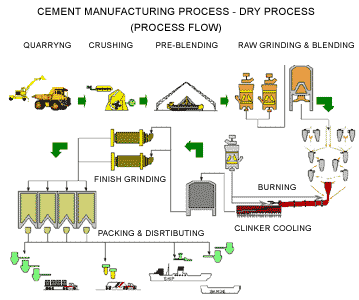
\includegraphics[scale=0.6]{process.png}
    \end{center}

    生产计划是关于企业生产运作系统总体方面的计划,是企业在计划期应达到的产品品种、质量、产量和产值等生产任务的计划和对产品生产进度的安排。它反映的并非某几个生产岗位或某一条生产线的生产活动,也并非产品生产的细节问题以及一些具体的机器设备、人力和其他生产资源的使用安排问题,而是指导企业计划期生产活动的纲领性方案。

\subsection {什么是生产计划}

    生产计划是指一方面为满足客户要求的三要素“交期、品质、成本”而计划;另一方面又使企业获得适当利益,而对生产的三要素“材料、人员、机器设备”的确切准备、分配及使用的计划。

    一个优化的生产计划必须具备以下三个特征:
        \begin{enumerate}
            \item  有利于充分利用销售机会,满足市场需求;
            \item  有利于充分利用盈利机会,实现生产成本最低化;
            \item  有利于充分利用生产资源,最大限度的减少生产资源的闲置和浪费。
        \end{enumerate}

    \subsubsection {生产计划的任务}

        \begin{enumerate}
            \item  要保证交货日期与生产量;
            \item  使企业维持同其生产能力相称的工作量(负荷)及适当开工率;
            \item  作为物料采购的基准依据;
            \item  将重要的产品或物料的库存量维持在适当水平;
            \item  对长期的增产计划,做人员与机械设备补充的安排。
        \end{enumerate}

    \subsubsection {生产计划的内容}

        \begin{enumerate}
            \item  生产什么东西—产品名称、零件名称;例:生产汽配行业的一种凸轮,名称代号:kj908
            \item  生产多少—数量或重量;因客人订单需要10000只,那实际生产应考虑到报废的产生,我们需要投产10500只,方能保证10000只的交货量。
            \item  在哪里生产—部门、单位;因生产制造行业的特性,显然我们主要是在生产部门完成指标,细化是在生产的各个工序班组间加工,包括:铸造、锻压、车床、铣床、高频淬火、磨床、清洗等。
            \item  要求什么时候完成—期间、交期。假如客人订单的交期要求在本月的20号,那么公司生产到完工应在20号之前完成,并且需要考虑物流运输的时间,以保证客户能在时限内收货。
        \end{enumerate}

    \subsubsection {生产计划的用途}

        \begin{enumerate}
            \item  物料需求计划的依据;
            \item  产能需求计划的依据;
            \item  其他相关计划的制定依据。
        \end{enumerate}

    \subsubsection {生产计划的种类}

        按不同性质划分,生产计划有各种类型见下表:

            \begin{itemize}
                \item  按时间周期分类
                    \begin{enumerate}
                        \item  2-3年长期计划,适用于产品群规划
                        \item  6-12月中期计划,适用于产品类别设计
                        \item  1-3月短期计划,是用于产品生产
                        \item  3-5周短期计划,适用于零件生产
                        \item  1-3日短期计划,适用于零件生产
                    \end{enumerate}

                \item  按计划层级/作用层级分类
                    \begin{enumerate}
                        \item  主生产计划(MPS)
                        \item  次生产计划(次MPS)
                    \end{enumerate}
            \end{itemize}

            此种分类常见与实际应用(尤其在有实体工厂的公司)。无论主、次生产计划(或主MPS、次MPS)其表现实体均是某个工序的计划安排。并选取其中最能体现公司经营运作和控制重点的工序作为其MPS(主MPS)的体现方式。一般制造业,均采用最后组装工序作为其MPS(主MPS)。

    \subsubsection {生产计划应满足的条件}
        \begin{enumerate}
            \item  计划应是综合考虑各有关因素的结果;
            \item  必须是有能力基础的生产计划;
            \item  计划的粗细必须符合活动的内容;
            \item  计划的下达必须在必要的时期。
        \end{enumerate}

\subsection {生产计划标准及层次}

    \subsubsection {生产计划的相关标准}

        \begin{enumerate}
            \item  作业计划的标准
                \begin{itemize}
                    \item  作业及加工的场所;例如:-------某某计划标准按照gb****** (当中的gb是指在中国境内生产的企业,*****是指行业名称);加工厂所可以是外协或本公司内生产,具体生产单位则是生产部。
                    \item  作业及加工的种类、顺序;例如:种类是指某种产品需要涉及到加工而产生的多少道工序,比喻上述所说凸轮加工,顺序则是指按完成凸轮制造而先做什么,后做什么,意思是将所有生产凸轮的工序进行排列。
                    \item  标准工时等。
                \end{itemize}

            \item  制程计划、余力计划的标准
                \begin{itemize}
                    \item  作业及加工制程别的负荷基准。
                    \item  作业及加工制程别的能力基准;制程计划是指制作与生产的工作程序,余力计划是指企业自身的生产能力与现有的生产能力差,比喻:本身企业每天生产1000只,那么现在我在生产800只,那么说明企业所提供的资源最大可以再生产200只,当超过总产量1000只,说明企业的生产能力饱和,这时如在增加生产那么我们必须相应增加设备与人力及各方面资源了。
                \end{itemize}

             \item  材料、零件计划的标准
                \begin{itemize}
                    \item  零件构成表及零件表;
                    \item  安排分区、供给分区;
                    \item  批量大小、产出率。
                \end{itemize}
            \item  日程计划的标准
                \begin{itemize}
                    \item  加工及装配基准日程表;
                    \item  批量。
                \end{itemize}
            \item  拟定库存计划的标准
                \begin{itemize}
                    \item  库存管理分区;
                    \item  订购周期;
                    \item  订购点、订购量;
                    \item  安全库存、最高库存、最低库存。
                \end{itemize}
        \end{enumerate}

        等等,上述计划标准,每逢变化时,应及时修正并予维持。

\subsection {生产计划指标}

    制定生产计划指标是生产计划的重要内容。为了有效的和全面的指导企业生产计划期的生产活动,生产计划应建立包括产品品种、产品质量、产品产量和产品产值的四类指标为主要内容的生产指标体系。

    1、产品品种指标

        产品品种指标是指企业在报告期内规定生产产品的名称、型号、规格和种类。它不仅反映企业对社会需求的满足能力,还反映了企业的专业化水平和管理水平。

        产品品种指标的确定首先要考虑市场需求和企业实力,按产品品种系列平衡法来确定。

    2、产品质量指标

        产品质量指标是衡量企业经济状况和技术发展水平的重要指标之一。产品质量受若干个质量控制参数控制。对质量参数的统一规定形成了质量技术标准,包括国际标准、国家标准、部颁标准、企业标准、企业内部标准等。

    3、产品产量指标

        产品产量指标是指企业在一定时期内生产的,并符合产品质量要求的实物数量。以实物量计算的产品产量,反映企业生产的发展水平,是制定和检查产量完成情况,分析各种产品质检比例关系和进行产品平衡分配,计算实物量生产指数的依据。

        确定产品产品指标主要采用盈亏平衡法、线性规划法等。

    4、产品产值指标

        产品产值指标是用货币表示的产量指标,能综合反映企业生产经营活动成果,以便进行不同行业间比较。根据具体内容和作用不同分为工业总产值、工业商品产值和工业增加值三种形式。

    生产计划的规划可以逐步精化为:

    \begin{enumerate}
        \item  无限能力计划。

      无限能力计划,指的就是在考虑出产计划、采购计划的时候,不考虑企业实际的出产能力,只管物料需求。这是大部门企业现在所采用的计划方法。这个方法的长处,就是操纵简便、轻易上手。但是,缺点也是很显著的。

        \begin{enumerate}
            \item  会增加企业的存货本钱。由于没有考虑到企业的实际出产能力,所以采购进来的良多材料,可能需要在企业中存一段时间才能用得着。要知道,这存放在企业里都是钱。放在企业中不仅会据有企业的资金,而且,对于企业的库存压力也不小,企业还要承担风险。如销售订单或者出产计划变更导致材料变为凝滞料的风险。
            \item  无法确定产品能否如期交货。由于没有考虑到企业的实际出产能力,所以,这个所谓的出产计划就会不断的进行变更。当一张出产订单由于产能的限制无法按时完成时,那其它的出产订单也不得不往后挪。所以,从无限能力计划上看不生产品能否及时交货。由于因为订单延期的不确定性,所以,最后,出产部分不得不像消防员一样,到处的去救火。
            \item  无限能力计划,不但会增加企业的存货本钱,而且会增加由于出产计划变更而造成的意外损失。企业若调整出产计划,则意味着还要调整职员铺排,有时候,可能因为产品的特殊性,还要调整出产线,那对企业的损失就大。
        \end{enumerate}

        \item  顺推法。

            顺推法指的是出产计划按照出产订单的前后逐一进行排。顺推法它考虑了企业的实际产能,所以,可以非常有效的解决由于无穷产能造成的题目。如企业可以根据出产计划来铺排采购计划及到料计划,从而减少企业库存的压力;由于考虑了实际产能,所以,基本上不会由于产能的题目而调整出产计划;同时,产品的交货期也有了一定的保障。但是,这个计划仍旧不是完美的,会出缺陷。
            \begin{enumerate}
                \item  若碰到紧急插单,就会无所适从。在企业中,根据客户重要性不同、产品的利润不同或者交货期的不同,紧急插单是常有的事情,特别是接单出产为主的企业。而顺推法的话,对于插单的敏感度不高。也就是说,利用顺推法把出产计划排好后,若碰到紧急订单的话,再重新排出产计划,那工作量会很大。一般企业的做法是,可能进行突击加班等手段,来解决这紧急订单的题目。
                \item  顺推法的工作量比较大。由于顺推法测算出产计划时,往往不能一次成功。有时候要在不同客户之间进行均衡、要最大程度的知足客户的交货需求,就需要不停的调整。而每调整一次出产计划,工作量都长短常大的。所以,利用顺推法进行出产计划排产的话,则灵活性会差良多。
            \end{enumerate}

        \item  计划模拟。

          第二种方法固然比第一种方法提高前辈,考虑了企业的产能。以上这两种排产的方法,使企业现在用的最多的。但是,由于其存在比较多的缺陷,所以,企业用起来,总觉得顾头顾不了脚,用其来不称心。就拿插单题目来说,就够他们头疼了。

            现在在实施项目的时候,一般建议用户用计划模拟的方法,来排产。由于前面两种方法太简朴,无法知足企业需求;而若用第四种方法,排程模块进行排程的话,对于企业的治理要求太高,企业可能无法合用。而用计划模拟的方法,可能更加适合企业。

            计划模拟简朴的来说,就是企业尺度产能与实际产能负荷进行对比,若实际产能负荷超过尺度产能的话,那就调整出产计划或者铺排职员加班增加企业尺度产能又或者委外加工出产。当然这个对比,若用手工来做的话,那工作量就长短常大的了。所以,要依赖ERP系统的匡助,来实现这个需求。

        \item  高级排程。

            在ERP系统泛起前,就有专门的排程工具,来匡助企业解决出产排程题目。但是因为其维护负责,所以,在出产企业中,也很难推广出来。

            利用高级排程工具,可以实现出产计划的顺排、到排,从而最大限度的知足企业的需求。实在,高级排程工具的原理,跟第三种方法是类似的,只是,第三种方法用的是手工,而第四种方法,是自动的。但是,由于企业治理的复杂性,所以,若想要全自动解决企业出产计划题目,那长短常难题的,对于企业的治理水平,也提出了比较高的要求。[1]
    \end{enumerate}

\subsection {主生产计划}

    生产计划是工厂管理内部运作的核心。一个优秀的工厂,其内部管理应该是围绕着生产计划来进行的。生产计划有月度计划、周计划、日计划。不过随着MRP的使用,“主生产计划”成为控制工厂内部运做的核心了。

    主生产计划(Master Production Schedule,简称MPS)

    一、MPS意义

    主生产计划是按时间分段方法,去计划企业将生产的最终产品的数量和交货期。主生产计划是一种先期生产计划,它给出了特定的项目或产品在每个计划周期的生产数量。一个有效的主生产计划是生产对客户需求的一种承诺,它充分利用企业资源,协调生产与市场,实现生产计划大纲中所表达的企业经营目标。主生产计划在计划管理中起“龙头”模块作用,它决定了后续的所有计划及制造行为的目标。在短期内作为物料需求计划、零件生产计划、订货优先级和短期能力需求计划的依据。在长期内作为估计本厂生产能力、仓储能力、技术人员、资金等资源需求的依据。

    二、MPS编制原则

    主生产计划是根据企业的能力确定要做的事情,通过均衡地安排生产实现生产规划的目标,使企业在客户服务水平、库存周转率和生产率方面都能得到提高,并及时更新、保持计划的切实可行和有效性。主生产计划中不能有超越可用物料和可能能力的项目。在编制主生产计划时,应遵循这样一些基本原则。

        \begin{itemize}
            \item  最少项目原则:用最少的项目数进行主生产计划的安排。如果MPS中的项目数过多,就会使预测和管理都变得困难。因此,要根据不同的制造环境,选取产品结构不同的级,进行主生产计划的编制。使得在产品结构这一级的制造和装配过程中,产品(或)部件选型的数目最少,以改进管理评审与控制。
            \item  独立具体原则:要列出实际的、具体的可构造项目,而不是一些项目组或计划清单项目。这些产品可分解成可识别的零件或组件。MPS应该列出实际的要采购或制造的项目,而不是计划清单项目。
            \item  关键项目原则:列出对生产能力、财务指标或关键材料有重大影响的项目。对生产能力有重大影响的项目,是指那些对生产和装配过程起重大影响的项目。如一些大批量项目,造成生产能力的瓶颈环节的项目或通过关键工作中心的项目。对财务指标而言,指的是与公司的利润效益最为关键的项目。如制造费用高,含有贵重部件,昂贵原材料,高费用的生产工艺或有特殊要求的部件项目。也包括那些作为公司主要利润来源的,相对不贵的项目。而对于关键材料而言,是指那些提前期很长或供应厂商有限的项目。
            \item  全面代表原则:计划的项目应尽可能全面代表企业的生产产品。MPS应覆盖被该MPS驱动的MRP程序中尽可能多数组件,反映关于制造设施,特别是瓶颈资源或关键工作中心尽可能多的信息。
            \item  适当裕量原则:留有适当余地,并考虑预防性维修设备的时间。可把预防性维修作为一个项目安排在MPS中,也可以按预防性维修的时间,减少工作中心的能力。
            \item  适当稳定原则:在有效的期限内应保持适当稳定。主生产计划制订后在有效的期限内应保持适当稳定,那种只按照主观愿望随意改动的做法,将会引起系统原有合理的正常的优先级计划的破坏,削弱系统的计划能力。
        \end{itemize}

    三、主生产计划的对象

    主生产计划的计划对象主要是把生产规划中的产品系列具体化以后的出厂产品,通称最终项目,所谓“最终项目”通常是独立需求件,对它的需求不依赖于对其他物料的需求而独立存在。但是由于计划范围和销售环境不同,作为计划对象的最终项目其含义也不完全相同。

    \subsubsection {编制生产计划的步骤}

    生产计划的编制必须遵循四个步骤

    (1)收集资料,分项研究。编制生产计划所需的资源信息和生产信息。
    (2)拟定优化计划方案统筹安排。初步确定各项生产计划指标,包括产量指标的优选和确定、质量指标的确定、产品品种的合理搭配、产品出产进度的合理安排。
    (3)编制计划草案做好生产计划的平衡工作。主要是生产指标与生产能力的平衡;测算企业主要生产设备和生产面积对生产任务的保证程度;生产任务与劳动力、物资供应、能源、生产技术准备能力之间的平衡;生产指标与资金、成本、利润等指标之间的平衡。
    (4)讨论修正与定稿报批通过综合平衡,对计划做适当调整,正确制定各项生产指标。报请总经理或上级主管部门批准。

    同时,生产计划的编制要注意全局性,效益性,平衡性,群众性,应变性。

\subsection {生产计划排程}

    生产计划排程的目的是为车间生成一个详细的短期生产计划。排产计划(Production schedule)指明了计划范围内的每一个定单在所需资源上的加工开始时间和结束时间,也即指出了在给定资源上定单的加工工序。排产计划可以通过直观的甘特图(Gantt-chart)形式给出。

    排产计划的计划间隔可以从一天到几周,取决于具体的工业生产部门。合理的计划长度取决于几个因素:一方面,它至少应当涵盖与一个定单在生产单元中最大的流动时间(flow time)相对应的时间间隔;另一方面,计划间隔受到已知顾客定单或可靠需求预测的可用性限制。很显然,只有当排产计划适度稳定时,在一个资源上进行定单排程才是有用的。也就是说,它们不应受不期望事件经常变化的影响(如定单数量改变或中断)。

    对某些生产类型(如jobshop),生产计划排程需要对(潜在)瓶颈资源上的任务定单进行排序和计划;而对另一些生产类型(如成组技术),生产计划排程要能自动地、按时段检查资源组的能力,看其是否能够在下一个时间段内完成成组加工的一组定单。然后,可以手工排序这组定单在下一个时间段内的加工次序。

    生产计划排程的安排应注意的原则:
    \begin{enumerate}
        \item  交货期先后原则:交期越短,交货时间越紧急的产品,越应安排在最早时间生产。
        \item  客户分类原则:客户有重点客户,一般客户之分,越重点的客户,其排程应越受到重视。如有的公司根据销售额按ABC法对客户进行分类,A类客户应受到最优先的待遇,B类次之。C类更次。
        \item  产能平衡原则:各生产线生产应顺畅,半成品生产线与成品生产线的生产速度应相同,机器负荷应考虑,不能产生生产瓶颈,出现停线待料事件。
        \item  工艺流程原则:工序越多的产品,制造时间愈长,应重点予以关注。
    \end{enumerate}

    排产计划任务能够而且也应当分散来做,这样可以利用每个地点人们的专业知识和车间当前状况的知识(例如人员的可用性)。

    生产计划排程受到上层主生产计划的约束,主生产计划设立了在分散的决策单位中执行生产计划排程的框架。从主计划中可获得的相应指导包括:使用超时或加班的数量;在不同时间点上来自供应链上游设施物料项的可用性;涉及来自供应商输入物料的采购协议。此外,由于主生产计划在供应链上有更宽的视点和更长的计划区间,从中我们还可以得到:
    \begin{itemize}
        \item  计划结束时需要建立的各物料项的季节性库存量;
        \item  交付给供应链下游设施的定单截止日期(下游设施可以是紧接着的下一级生产单位,分销商或最终顾客)。
    \end{itemize}

    生产计划排程的安排应注意的原则:

    \begin{enumerate}
        \item  交货期先后原则:交期越短,交货时间越紧急的产品,越应安排在最早时间生产。
        \item  客户分类原则:客户有重点客户,一般客户之分,越重点的客户,其排程应越受到重视。如有的公司根据销售额按ABC法对客户进行分类,A类客户应受到最优先的待遇,B类次之。C类更次。
        \item  产能平衡原则:各生产线生产应顺畅,半成品生产线与成品生产线的生产速度应相同,机器负荷应考虑,不能产生生产瓶颈,出现停线待料事件。
        \item  工艺流程原则:工序越多的产品,制造时间愈长,应重点予以关注。
    \end{enumerate}

\subsubsection {生产计划管理的作用}

    生产计划对合理均衡地组织生产,提高企业经济效益有着极其重要的作用。具体说有如下几点:
    \begin{enumerate}
        \item  生产计划是日常生产活动的依据,可使企业各生产环节和全体员工统一、协调动作,充分利用人力和设备,使企业各环节有组织地、系统地进行。
       \item  可使企业均衡的、有节奏的组织生产。均衡稳定的生产,是提高劳动生产率,保证产品质量,降低产品成本,保证安全生产的重要手段。组织均衡生产是生产计划的原则和任务,各生产环节只有按作业计划组织生产,才能使生产均衡地进行,同时编制生产计划也可以综合反映企业的技术和管理水平。
        \item  生产计划是联系供、产、销、运等日常工作和日常生产技术准备工作的纽带,通过它可以把企业日常生产经营活动组织起来。
        \item  生产计划是组织企业生产活动不断平衡的手段。企业在生产活动过程中,各部门、各生产环节之间会经常出现新的情况、新的矛盾,即经常会打破原来建立起来的相对平衡。生产计划是短期计划,它可以根据这些新情况、新矛盾和新问题来安排生产环节的任务,建立起新的相对平衡关系,保证生产的顺利进行。
    \end{enumerate}
 %  生产计划
    \section {采购订单管理}

    采购订单是存货在采购业务中流动的起点,是详细记录企业物流的循环流动轨迹、累积企业管理决策所需要的经营运作信息的关键。通过它可以直接向供应商订货并可查询采购订单的收货情况和订单执行状况,通过采购订单的关联跟踪,采购业务的处理过程可以一目了然。

    采购订单标明了
        \begin{itemize}
            \item  供应商
            \item  要订购的物料或服务
            \item  数量
            \item  价格
            \item  供货日期和供货条款
            \item  支付条款
        \end{itemize}
    此外,采购订单确定订购的物料是存入库存还是在收货时就直接被消耗。采购订单须经核准。

\subsection {采购订单的分单}

        采购业务的目标,一是满足对物料的需求,二是降低成本,第三还包括质量,质量是采购业务能够发生的前提条件,肯定要满足。在采购管理中还有一个重要管理内容,那就是如何做内控,因为采购往往是企业花钱最多的部门,内控做得不好,最终影响产品成本和质量。

        订单分配是采购管理的一个核心问题,也是一个难题,因为分单需要综合平衡内外各种关系以实现采购业务目标,同时还要加强内控。假设采购一种物料N吨,有三个供应商ABC,如何给三个供应商分采购量?

    \subsubsection {策略方式一}

        80/20方法。绝大部分给A企业(例如80\%),另外小部分给另外B企业,或者B、C企业;这样做的好处是绝大部分订单量给A,可以获得批量经济折扣,获得更低成本。B、C做为培养关系的供应商,在A出问题时候可以快速补充,相当于备份的大供应商,可以避免供应中断。

        这种操作方式存在一种内控上的难题,最大的采购量到底给哪一家?面向各个供应商采购不同的量,采购价格如何确定?供应商可以通过向采购决策人公关以获取最大的采购量,而供应量小的供应商也可以公关获得好的采购价格,因为量不一样,价格和采购量大的不能完全比较。实际上大小供应商都有发挥空间。

        解决的方法:通过供应商评估确定优先供应商,备份供应商,明确主供应商和备份供应商的量的分配比例原则,减少了第一层次的内控(不过,这需要定期评估,以评估小组操作);第二层次的内控,那只有参考市场价格了,很难内控;或许可以通过对采购人员整体部门KPI的相关考核来加强内控,比如考核年采购成本降低金额等。

    \subsubsection {策略方式二}

        平分方法。一些企业的分单策略是平分:采购订单在三个供应商之间平分,这是一个非常简单的处理原则,很容易操作,很容易检查。

        操作过程:采购量在三个供应商之间平分。在了解市场价格基础上,和三个供应商谈判价格,取三个供应商价格最低者,要求另外两家也达到最低价格(因为别的供应商能够达到,要求你达到这个价格是合理要求);在谈判中的策略是:“A供应商已经做到10元了,B你也应该可以做到10元。”在和B谈判妥当的时候,三家供应商一起签订合同,和三家供应商价格大家都能够看到,有一定的透明性,证明不是压价策略。这种谈判最多做一轮,不会重复要求供应商压价。出价高的供应商晚获得订单,如果不降价,失去订单也是可能的。

        策略分析:这样做的原因很重要一点是加强内控。采购内控主要有两个点:一是决定哪个供应商可以入围成为合格供应商,另外一个是分单多少。入围合格供应商是产品开发部门确定的,一次性的;分单是经常性的,是内控重点。采取平分原则,则是的分单透明化,供应商不用公关,可以减少公关成本,消除一个在订单数量分配上的内控问题。其次三个供应商均要求实现最低价,消除在价格上的内控问题。如果供应商在数量和价格上均是凭实力,不需要公关,那么成为企业的合格供应商也需要凭实力,即使不能完全消除第一个方面内控问题(成为合格供应商)也关系不大,毕竟只是一次性的事情。

        看来,这种貌似不好的分单策略(不能获得规模效益),还有深刻的内控优势,也是一个不错的策略。当然,应用这个策略的企业还未规范开展供应商管理,假如有规范的供应商管理,这是否是一种好的策略,值得探讨。

\subsection {采购订单的更新控制}

    虽然系统会自动根据采购计划生成采购订单,但是在实际工作中,采购员往往还需要对采购订单中的部分内容进行更新。为了加强控制,无疑需要对这个更新作业进行更细致、更深入的管理。那么在采购订单中更新部分内容会触发那些业务逻辑呢?笔者在这里根据自己的了解作一番分析。希望这个分析报告可以帮助大家更加深入的了解单据的更新操作。

    采购订单中有很多内容都是从产品基本信息表中取得。如产品的规格描述、产品的计量单位、产品的包装要求等等。有时候企业根据实际需要,可能需要在采购订单上更新这些信息。如以前供应商送原材料过来的时候是4个一包的。现在企业为了某种原因,如生产线的要求,需要把这个包装数量改为3个一包或者5个一包。此时,在采购订单的包装说明中可以进行更改。更改保存后,就完事了吗?其实,这背后还暗藏着一个业务逻辑。即这个包装信息、产品规格等等属于产品的基本信息范畴。那么在采购订单上进行更改后,是否要求采购订单在保存更新的同时去更新产品基本信息表中的内容吗?还是只是采购订单上更新即可?

    到底采用什么方式,主要根据企业业务性质来判断的。如果这个更新只是一个临时的调整,那么就不需要更新产品基本信息中的内容。但是,如果这个更新是永久的,以后都要采用这个包装方式的话,则就需要在更新采购订单的同时更新产品基本信息表中的内容。不过产品基本信息表中的内容毕竟比较敏感,如果想通过订单关联更新产品基本信息表中的内容,则要符合一些业务逻辑的控制规则。具体来说,主要有三个方面。

    \begin{enumerate}
        \item  产品信息表中必须指明某个字段可以被其他单据所更改。

        这主要是为了保证数据的一致性。因为在企业中,原材料等基本信息往往不是采购人员建立,而是研发部门等建立。为此,研发部门有这个权利那些内容可以被其他人员更改。如此的话,当其他部门通过其他单据更改了某部分内容之后,作为产品信息的主人,就比较容易追踪。在实际工作中,笔者建议企业用户,把一些关系不是很大的内容,如包装方式等等可以让其他员工进行更改,以减少信息建立人员的工作量。但是,对于一些关键的参数,如原材料检验标准、原材料规格等字段的话,最好还是谁建立谁更改。

        \item  用户需要有这张表对应的权限

        如在ERP系统权限设计中有一个排它权限。如果某个用户做了这个限制之后,则他建立的信息可能就只有他自己能够进行更改。其他用户无权进行修改。如果有这个限制的话,则其他用户就无法通过采购订单等相关单据更新这个产品基本信息表。

        \item  是采购订单中的控制

        在实际工作中,可能需要更新与不需要更新两种情况同时存在。是否需要更新产品基本信息表的内容需要采购员根据实际情况来进行判断。为此,在采购订单更新用户按保存后,系统就会进行判断。更改的内容是否涉及到产品基本信息表中的内容。如果涉及到而且产品基本信息表中又指定这个字段可以被更改的话,则系统就会提示用户是否需要把这个更新同步到产品基本信息表中。如果用户选择是的话,则这个更新会被同步到产品基本信息表中。如果选择否的话,则只是在采购订单上进行更新,而不会涉及到产品基本信息表。
    \end{enumerate}

    也就是说,要同时满足以上三个条件,产品基本信息表中的内容才能够被采购订单所更新。笔者在项目推广中,对于用户的建议是这个功能要慎用。对于一些共享程度比较高的信息可以通过级联更新来节省数据维护的工作量。但是对于一些技术性比较强的数据,则最好还是采取专人维护专人负责制比较好。
与产品价格信息表关系

    除了会对采购订单中的产品基本信息如包装信息进行更改,采购员改的最多的还要算是采购订单价格。这个采购订单价格在采购订单管理中又是一个比较敏感的字段。为了保障企业资金的安全性,采购订单在这个字段的更新上采取了比较多的控制措施。
    \begin{enumerate}

        \item  采购订单价格更新

        首先,采购订单会控制采购员是否有这个权限更改这个采购价格以及更改的幅度有多大。有些企业对于这个采购价格控制的比较严格,普通采购员无法更改这个采购价格。因为采购订单中的价格自动会从供应商产品价格表中带出来。也就是说,默认的价格就是跟供应商协商好的价格。若要进行价格变动的话,则必须由采购经理来完成。有些企业则相对宽松一点,采购员可以更改采购订单的价格,但是其有一个幅度的限制。如某个原材料标准价格为10元,而采购员可以在1\%的范围内修改这个采购价格。也就是说,其向供应商采购时,其价格的最大修改权利只有11元。如果超过这个价格的话,就需要采购经理或者其他人员的授权才行。可见通过对采购价格这个字段本身的权限控制,能够大大的提高采购订单价格的准确性。明显消除采购员与供应商串通的徇私舞弊行为。

        \item  采购订单价格更新对其他数据表的影响

        采购订单的价格更新是否会对其他相关表产生影响呢?这里的相关表主要包括两张数据表,分别为产品价格信息表与产品供应商价格信息表。产品价格信息表中定义了产品的计划价格;产品供应商价格信息表则定义了某个供应商的具体价格信息。他们之间有彼此的联系。如产品供应商价格信息表默认情况下,会继承产品计划价格表中的价格。而在建立采购订单的时候,默认情况下其价格来自于产品供应商价格信息表。如果这张表中没有相应数据的话,则其会采用产品计划价格表中内容。而现在反过来,如果采购订单中物料价格的变化,是否会更新以上这些表中的内容呢?
    \end{enumerate}

    笔者在项目实施中,给用户第一个建议是最好不要通过采购订单来更新这两张基本价格表中的信息。若产品计划价格表中或者供应商价格信息表中的内容有改变的话,最好通过独立的变更单据来进行变更。这主要是出于数据的一致性考虑。而且也易于后续的查询追踪。如果在采购订单中进行级联更新的话,以后很难查询到这个更改记录。虽然这会增加一些数据维护的工作量。但是却可以保持数据的一致性,笔者认为这个交易还是值得的。

    \textbf {建议}

    笔者给用户的第二个建议是如果供应商价格变化真的很频繁。就像前一段时间,原材料的价格几乎是一月一变。在这种情况下,如果每次价格变化时都要先更改供应商价格信息表中的内容,那显然工作量会变得很大。而每次去更改采购订单的价格也不利于采购订单的管理。对于这种情况,如果原材料市场价格变换比较频繁,那么笔者建议企业用户,可以让采购订单更改供应商价格信息表,但是级联更新只限于此,而不能够更改产品基本价格表。因为产品基本价格表不仅跟采购订单或者供应商价格表相关;而且还是计划成本计算的来源。而产品计划成本在一段时间内必须是稳定的。如故其也是随着市场价格波动而波动的话,就不利于进行计划成本与实际成本的对比分析。故在任何情况下,产品基本价格表的信息都不能够通过采购订单或者采购订单变更单来更新。而只能够通过独立的单据来进行更新。

    而且,产品标准价格表中的价格信息也不能够经常变更。最好其更改的频率不要超过每月一次。否则的话,会导致计划成本的不稳定。不利于后续的统计分析。同时,也会增加维护的工作量。如笔者有一家客户,即使在价格变动频繁的市场环境中,其原材料计划价格也是一个季度调整一次。

    由于采购订单中价格更新涉及到三个层次的价格表信息,所以更新控制就会更加的严格。笔者维护的多个ERP项目中,其用的最多的控制方式如下:

    \begin{enumerate}
        \item  在采购订单控制上,采购员可以更改价格。但是其更改后的价格不能够超过供应商基本价格表中的价格。也就是说,采购员降低采购价格是允许的,但是若要调高采购价格则是不允许的。并且系统会有一张采购订单实际价格与供应商价格信息表的分析报表,用来对采购员进行考核。

        \item  采购订单价格更新一般情况下不会更新其他基础价格表中的内容。最多只是更改供应商价格表中的价格信息。
    \end{enumerate}
 % 采购订单
    \section {询价采购}

    询价采购,是指询价小组(由采购人的代表和有关专家共3人以上的单数组成,其中专家的人数不得少于成员总数的三分之二)根据采购需求,从符合相应资格条件的供应商名单中确定不少于三家的供应商向其发出询价单让其报价,由供应商一次报出不得更改的报价,然后询价小组在报价的基础上进行比较,并确定最优供应商的一种采购方式,也就是我们通常所说的货比三家,它是一种相对简单而又快速的采购方式。政府采购法规定实行询价采购方式的,应符合采购的货物规格、标准统一、现货货源充足且价格变化幅度小的政府采购项目。

    询价采购有如下几种类型:
        \begin{itemize}
        \item  询价采购还可分为报价采购、议价采购和订购。
        \item  报价采购是指采购方向供应商发出询价或征购函,请其正式报价的一种采购方法。
        \item  议价采购是指与供应商进行个别谈判,商定价格的一种采购方法。
        \item  订购是指利用订购单或订购函,列出采购所需物资及标准寄给供应商的一种采购方法。
        \end{itemize}

\subsection {询价采购过程}

    询价采购的具体过程如下:
    \begin{enumerate}
        \item  成立询价小组。

        这是执行询价采购方式的重要环节,询价小组由采购人的代表和有关专家共3人以上的单数组成,其中专家的人数不得少于成员总数的 2/3。要选择专业水平较高、素质全面的人士参加,专家组成的询价小组应对采购项目的价格构成和评定、成交标准等事项做出规定。询价小组根据所要采购的内容选定从符合相应价格条件下的供应商名单中选定3家以上的供应商,并且为询价采购做好充分的事前准备,如确定采购的需求、预测采购的风险等等。

        \item  确定被询价的供应商名单。

        询价小组根据所采购商品的特点及对供应商、承包商或服务提供者的要求,特别是根据要采购的内容,从符合相应资格条件的供应商名单中,选定3者以上的供应商。选择时必须依据所要采购的内容,同时考察各供应商的供应能力和资格条件,做出慎重选择。

        \item  询价。

        对所选定的供应商分别发出询价单,询价单的内容除了价格以外,还应包括商品品质、数量、规格、交货时间、交货方式、售后服务等内容,供应商应就询价单的内容如实填报。询价小组要求被询价的供应商一次报出不得更改的价格。这适用于采购现成的而并非按采购人要求的特定规格特别制造或提供的标准化货物,货源丰富且价格弹性变化不大的采购项目;在询价采购实践中,存在着与采购人等有串通现象,报出的价格不符合市场经济规律性;甚至出现有特殊的供应商报价后又更改的不良倾向。所以,这就要求询价小组一定要规范供应商的报价,坚持依法规定一次性报价;没有更改的机会,切防相互之的勾结腐败行为。

        \item  确定成交供应商。

        采购人根据符合采购需求、质量和服务相等且报价最低的原则确定成交供应商,并将结果通知所有被询价的未成交的供应商。采购人要在依法、科学、规范化地情况下进行;

          \begin{enumerate}
              \item  询价小组完成询价工作后,要形成询价报告,提交给采购人;
              \item  采购人要依法、科学、规范化地进行供应商的成交确定;
              \item  采购人在确定成交供应商时,必须严格执行事先确定的成交供应商评定标准;
              \item  采购人确定成交供应商后,要将结果通知所有被询价的未成交供应商。
            \end{enumerate}
    \end{enumerate}

\subsection {询价采购的风险形式}

    \begin{enumerate}
    \item  价格风险。

        询价采购遵循的是货比三家,通过多家供应商之间的竞争获取质优价廉的物品,但由于信息不对称的存在,加之询价采购报价方式的缺陷,导致了采购过程中的价格风险,具体表现为以下几个方面:一是价格垄断。市场经济的飞速发展,使得一批产品质量过硬、品牌信誉高的企业脱颖而出,这类企业往往是一些大型企业,具备完善的销售渠道和营销体系,在某个城市和地区都设有总代理商,掌握了一定区域市场价格的话语权,这使得在采购此类产品时,采购机构所询价的供应商都向总代理商申请特价,无形中形成了一个价格垄断体系,最终询价的对象实质上只有一家,即某品牌产品的地区总代理商,表面上公开.公平的询价采购只能流于形式,无法有效实现通过价格竞争获取最优价格的功能。

        合谋报价。合谋报价是指被询价的供应商互通信息,联手操纵价格给集中采购带来的风险。从笔者参与的多次询价采购来看,以办公自动化产品为例,由于被询价的供应商所在的地域相对集中,相互之间常有调剂产品的现象发生,某些供应商之间会达成一定的策略同盟,在回应采购机构的询价时会私下达成协议,促成某个供应商赢得采购合同,不难想见,此时所获取的价格就不是最优价格,这给集中采购的效益蒙上了一层阴影。

        低价陷阱。低价陷阱是指某些供应商为赢得采购合同和提供售后价策略,但在执行合同和提供售后服务上大打折扣,给采购的后续环节带来许多不确定因素,影响了采购整体效益的提高。从采购实践来看,此类风险在询价采购中并不鲜见,某些供应商在询价单上报出低价后,在执行合同时却以各种理由推脱,如无法按期交货、产品的配件或附加设备不全,有的甚至以次充优,偷梁换柱,给询价采购带来了隐患。

    \item  采购机构的道德风险

        由于信息不对称的普遍存在,询价采购中采购机构的道德风险也是不容回避的问题,采购机构的道德风险是指采购机构利用供应商所不知道的私有信息采取不利于供应商的行为,在询价采购中主要表现为:一是采购信息的不公开。在询价采购中,采购机构出于机构利益或个人利益的考虑,对本应公开的信息隐而不发,使某些具备实力的供应商失去参与机会,损害了潜在供应商的知情权。二是保护主义引发的对供应商的歧视政策。在采购活动中,采购机构往往出于保护老客户和本地关系户的目的,在制定询价采购方案和沟通采购信息方面对熟悉的供应商给予倾斜照顾,无形中造成了对外地供应商和潜在供应商的歧视,影响了供应商之间的公平竞争。三是确定询价供应商过程中的暗箱操作。《政府采购法》规定,确定供应商的程序、标准、依据等应该及时向供应商公布,然而在实际工作中,采购机构可能采取拖延信息发布,模糊选择标准等办法给供应商知晓信息造成壁垒,从而为确定询价供应商中的暗箱操作创造机会。

    \item  询价流程的失范风险

        现行《政府采购法》对询价采购的具体操作流程没有规范,各单位在进行询价采购时的程序各不相同,价流程缺乏统一性和规范性,这使得询价采购可能存在失范风险,影响了采购效益的提高。一是询价对象选择过程的失范。确定询价对象是询价采购的首要环节,也是影响询价采购效益的重要因素,在具体采购活动中,由于没有相关法律条文规范询价对象的选取方式,各单位在选取询价对象时的方法不尽相同,有的从熟悉的供应商中挑选,有的从以往打过交道的供应商中选取,没能较好体现询价对象选择的公开透明,对潜在合格供应商造成了一定的歧视。二是报价过程的失范。供应商在回应采购机构的询价时往往采取的是传真方式,由于各供应商报价时间不一,有些供应商便企图利用报价时间差获取其他供应商的报价信息,以调整自己的报价,影响了最优采购价格的实现。三是供应商评定标准的失范。在确定预成交供应商时,通常采取的是最低价法,即报价最低的供应商赢得采购合同,但在实际与机会,损害了潜在供应商的知情光采购画上了一个问号,这需要从询操作中,某些供应商虽然报价很低,但全寿命采购理念来看,此类供应商是不可取的,因此亟需从法规的角度规范供应商的评定标准,确保“物有所目标的实现。

    \item  供应商履约风险

        询价采购具有采购周期短的优点,但换个角度考虑,正是由于其组织设计上的缺陷,无法在事前和事中对供应商进行全面细致的考察,为后续履约环节埋下了隐患,表现在实际采购活动中,则是供应商在以低价获得采购合同后,却不能按期或保质保量地履行合同,主要体现在:一是有价无货,在笔者参与的多次询价采购中,有时供应商在以低价成为预成交商后,却以暂时无货为理由拒签合同,给采购任务的完成制造障碍;二是低价劣货,由于信息不对称,供应商在供货时往往采取以劣充优,以次充好来蒙蔽往往采取以劣充优,以次充好来蒙蔽用户,这类货物往往是返修率和故障率双高,造成了用户对采购机构的不满三是售后服务大打折扣,某些供应商在履行售后服务义务时往往推三阻四,以各种理由降低服务质量,使得所购产品的服务质量无法得到保障。

    \end{enumerate}

\subsection {询价采购风险的防范对策}

        询价采购的风险一定程度上给阳价采购制度和运行机制等方面加以完善和防范,以促进政府采购健康有序地发展。

    \begin{enumerate}
    \item  加强供应商资质审查,合理选择询价对象

        供应商资质审查是询价采购的一个重要环节,只有所询价的供应商均是资质优良、诚信良好的企业,才能有效地化解后续采购风险的发生,保证采购质量。但由于询价采购周期短,而供应商的资质却是一个长期的系统的考察过程,不可能在短期内对某个供应商的资质做出准确的评判,这就需要采购机构立足平时,做实做细这项工作。一是要建立完备的供应商数据库,供应商资料的收集非一朝一夕之功,需要采购机构在每次采购完成后,及时整理参与采购的供应商资料,按照产品分类建立相关供应商数据库,定期对产品市场进行考察,掌握产品的主要品牌、主要生产企业和区域总代理商。二是可以采取供应商资质年审制度。供应商资质年审制度符合供应商动态管理的要求,采购机构每年初可在指定媒体上发布年审公告,注明供应商所需呈交的资质材料,而后组织相关领域的专家对供应商进行评定,对供应商实施分级分类管理。三是加强与中介机构的信息沟通。某些行业协会或诚信评估机构对供应商的了解是非常全面的,采购机构应加强与此类机构的横向协作和信息沟通,既可以及时掌握丰富翔实的供应商资料,还能大大减少信息收集成本,可以有效提高供应商资质审查的效益。

    \item  建立健全采购机构内部监督制约机制

        采购机构内部监督制约机制的完善是有效防范采购机构道德风险的一剂良方,只有从制度上堵住采购人员徇私舞弊的入口,才能确保询价采购的公开、公正和公平。建立健全采购机构内部监督制约机制,一是要科学分工,明晰职责,在采购机构内部建立起分工协作、相互制约的工作机制。每次询价采购前要成立询价小组,小组应由包括采购人员和有关专家在内的三人以上单数构成,小组在询价前要明确各人分工、询价供应商的资质标准及选取方式,评价成交供应商的标准以及合同管理办法等。询价小组的运作要保证相互牵制、协调高效,以杜绝采购中可能出现的"一言堂"和暗箱操作。二是要充分发挥纪检审价部门的作用,采购机构内部的纪检审价人员应参与询价采购的整个流程,监督询价采购的各个环节是否按规程运作,在供应商选择和供应商评定等敏感环节是否有舞弊行为发生,最后确定的成交价是否合理等,以保证对询价采购的实时有效监督。

    \item  规范询价采购流程

        规范的询价采购流程是询价采购健康发展的关键所在,只有询价采购流程实现了规范化、制度化,才能有效提高采购效益。一是要明确询价对象的选取方式,按照"三公"原则的要求,采购机构应对所有资质合格的供应商一视同仁,确保机会均等,基于采购成本的考虑,不可能对所有供应商进行询价,因此在资质合格的供应商库中,只有通过随机抽取的方式,才能保证询价对象选取的公正。二是规范供应商报价过程。要有效杜绝供应商利用时间差获取其他供应商报价信息,必须规定所有被询价供应商在规定时间以密封形式报价,然后由询价小组统一拆封,进行比价。三是科学合理地制定供应商评定标准,要从全寿命角度考虑产品的成本,确保所采购产品在寿命期间内性价比最高。

    \item  发展与供应商的合作伙伴关系

        发展与供应商的合作伙伴关系是采购机构供应商管理内容上一次质的飞跃,通过建立采购机构与供应商之间共享信息、共担风险、共同获利的合作伙伴关系,可以有效降低双方之间的信息不对称程度,抑制询价采购中供应商违约等不利行为的发生。在合作伙伴关系建立的过程中,需要重点解决好以下几个问题:

        \begin{itemize}
            \item  充分利用同实施监督与激励。采购合同是供应商和采购机构为进行产品交易而签订的明确双方权利义务的书面协议,具有法律效力。在设计合同条款时,采购机构应充分考虑合作中可能出现的意外情况,如产品成本控制不力、交货不反时、产品质量有缺陆等。在合同中明确出现此类情况时的处理方式反双方责任、风险的分担。

            \item  参与供应商的长期规划,增加其有害选择的机会成本。采购机构通过参与供应商的长期规划,不仅可以加深相互的了解,而且使供应商相信长期合作的真实性,在其选择不利行为时,会充分考虑行为造成的对其长期利益的损害,增加这种有害选择的机会成本,保证双赢结果的实现。

            \item  及时收集用户反馈信息,加强对供应商监督。采购机构应当定期收集用户对供应商供货情况、产品质量情况和售后服务情况的反馈意见,井要求供应商&时处理。对一些可观测的供应商行为,如产品质量控制、产品交付能力等,采购机构可采取定期检查或抽查等形式,如供应商不符合标准,则采取相应的惩罚措施。对不可观泪IJ的供应商行为,如技术创新、产品成本控制等,可根据实际结果设计奖励合同,充分调动其改革积极性。

        \end{itemize}
    \end{enumerate.zh}

\subsection {询价采购的注意事项}

    第一,最大程度地公开询价信息。参照公开招标做法,金额较大或技术复杂的询价项目,其采购信息也应在省级、中央级媒体上发布,最起码应当在地级市的党报、采购网、电视台发布,扩大询价信息的知晓率,信息发布要保证时效性,让供应商有足够的响应时间,询价结果也应及时公布。通过公开信息从源头上减少“消息迟滞型”“不速之客”现象的出现。

    第二,更多地邀请符合条件的供应商参加询价。被询价对象确定要由询价小组集体确定。询价小组应根据采购需求,从符合相应资格条件的供应商名单确定不少于三家的供应商,被询价对象的数量不能仅满足三家的要求,力求让更多的符合条件的供应商参加到询价活动中来,以增加询价竞争的激烈程度。推行网上询价、传真报价、电话询价等多种询价方式,让路途较远不便亲来现场的供应商也能参加询价。

    第三,实质响应的供应商并非要拘泥于“三家以上”。政府采购法规定,只要发出询价邀请的供应商达三家以上即可,前来参加并对询价文件作实质响应的供应商并非要人为硬性地达到三家,但是起码要达到两家以上,询价采购由于项目一般较小往往让大牌供应商提不起兴趣,如果非得要达三家,询价极可能陷入“僵局”,重要的是要形成竞争,而非在供应商数量上斤斤计较。

    第四,不得定牌采购。指定品牌询价是询价采购中的最大弊病,并由此带来操控市场价格和货源等一系列连锁反应,在询价采购中定项目定配置定质量定服务而不定品牌,真正引入品牌竞争,将沉重打击陪询串标行为,让“木偶型”“不速之客”绝迹于询价采购活动,让采购人真正享用到政府采购带来的质优价廉的好东西。

    第五,不单纯以价格取舍供应商。法律规定“采购人根据符合采购需求、质量和服务相等且报价最低的原则确定成交供应商”,这是询价采购成交供应商确定的基本原则,但是不少人片面地认为既然是询价嘛,那么谁价格低谁“中标”,供应商在恶性的“价格战”中获利无几,忽视产品的质量和售后服务。过低的价格是以牺牲可靠的产品质量和良好的售后服务为条件的,无论是采购人还是供应商都应理性地对待价格问题。不可否认,价格是询价中的关键因素,但绝非惟一因素,在成交供应商确定上要综合评审比较价格、技术性指标和售后服务等,在此基础上依法确定。

\subsubsection {以“价格”论英雄 不是竞价采购与询价采购的初衷}

    在以买方市场为主的现实经济环境下,不管是采购企业还是供应商都在想方设法降低企业的生产与管理成本,以提高自身企业的市场竞争力。开始有一些企业应用网上竞价采购与询价采购的电子商务模式,然而有部分企业在使用竞价采购平台和询价采购时在最终评审过程中,存在仅以价格定标的现象,产生了产品质量与后继服务跟上等一些问题。而出现的这些现象并不是我们设计询价支持系统所想看到的,设计初衷是为了企业通过竞价采购平台从更多的优质供应商中找到最优价格的供应商,而非最低价的供应商。

      在实际的竞价平台的具体运用中,不少企业在实施“竞价采购平台”与“询价采购平台”时,往往只重视“价格”指标,看谁的“报价”低,就让谁中标。这不仅引起了不少供应商的异议,一些采购人也因中标商的后续服务不力等而不满这种采购行为。即使是竞价与询价采购,也不能仅仅以“价格”作为唯一的评标标准。

      一、以“价格”论英雄的危害性

    \begin{enumerate}
        \item  容易造成被询价对象低价抢标,进而影响到采购项目的质量。

        从客观上讲,对政府采购这块蛋糕,没有一个供应商不是垂涎欲滴的,谁都想中标,也都想赚钱,这是他们办企业搞经营的目的和宗旨。而在实际工作中,不少的采购企业及其采购代理机构却偏偏就是以供应商的“报价”来作为评定他们中标与否的唯一依据,这就“迫使”被询价供应商要想中标,就只能降低报价,并且也只能从“价格”指标上去“努力”,才能提升他们的“竞争力”。对此,不少的供应商面对“难得”的被询价机遇,他们就只能采用“低价”的手段去抢标,而不想过多去考虑这宗供应业务是否能“赚”多少钱,甚至于暂时也不考虑是否能赚钱,取得中标资格是首位的,而一旦他们中标后,就开始算起“细账”,项目供应就全部围绕其“赚钱”的目的,并大肆削减项目的供应成本,不是变相减低项目的配置标准,就是减少附件功能,或是采用低质甚至于劣质材料等措施,结果,采购项目的质量肯定受到严重的影响,产品的使用寿命也必将因此而下降,采购人的权益受到了很大的侵害。这就是以“低价”论英雄带来的弊端。

        \item  容易造成中标商后续服务不力,导致采购人权益难以得到保障。

        正是由于采购人或其采购代理机构对采购项目中标条件的确认,过分地集中在供应商的“报价”上,而不少的供应商在竞标时,为了能够中标,在“价格方面也已“被迫”作出了较大的“让步”,因此,他们在中标后,就不会再关心供应项目的后续服务了,因为,一方面是采购人自己没有将“服务”等指标提高到应有的重视程度,供应商就更不会主动去服务;另一方面,中标商也要赚钱,在较低的中标价位下,再持续提供那些“免费”服务,必然加大额外的成本开支。因此,如果单单就以“价格”论英雄,就必然会导致采购人得不到周到的后续服务。

        \item  容易造成企业采购只是追求资金节约的假象,进而影响企业采购形象。

        众所周知,企业采购的目的和宗旨不仅仅是为了节约采购资金,提高财政资金的使用效率,而是还必须要考虑到其他诸多的因素,如维护国家和社会利益、保护环境、保障当事人的正当权益等。而询价采购又是一种使用频率较高的企业采购方式。据不完全了解,在不少的县、市,有85\%以上的采购项目都是通过“询价”方式采购的,因此,如果对待仅仅“价格”来判断或认定供应商中标与否,势必就会给供应商造成一种企业采购的宗旨就是为了追求资金节约率,而不顾供应商应分享的利润,更不顾其他当事人正当权益的错觉,这就弯曲了企业采购的宗旨,直接影响了企业采购的外在形象。
    \end{enumerate}

    二、防范仅以“价格”指标作为中标条件的根本措施

    \begin{enumerate}
        \item  科学设置评标指标“体系”,杜绝以“价格”为单一评标标准。采购代理机构为采购人代理任何一个采购项目时,都应同时为采购人考虑到以下几个关键性的指标参数:

        \begin{itemize}
            \item  价格指标,即投标人(被询价人)对采购项目的报价情况,这是衡量采购资金使用效率(即节约额)的重要指标;
            \item  服务指标,即被询价人为采购人提供的售后服务工作,这是衡量采购人权益保障程度的重要指标;
            \item  质量要求,即对采购项目配置、性能等提出的具体要求;
            \item  采购人的需求,对任何一个采购项目,其质量、标准、配置等有高有低,档次有高、中、下,产品功能也有多有少等等,但是否适合于特定采购人的需求,还必须由采购人根据具体情况而定。
        \end{itemize}

        这些都是与采购人权益息息相关的缺一不可的重要指标,因此,作为用来评标的标准就必须要围绕这些基本因素来展开,针对不同采购人的具体情况,分清各个指标的轻重程度,采取综合评分法,评定出各供应商的综合竞争力,而不能仅仅以“价格”作为唯一的评标因素。

        \item  全面公示评标结果,遏制片面追求低价的采购行为。众所周知,询价采购是企业采购活动中常用的一种采购手段,但其不属于也不同于公开招标的采购方式,相对来说,询价采购的不少必要环节和特定的操作步骤都是在比较小的范围内实施的,这样,只有对询价采购过程中的相关信息充分对外公开,才能有效提高其采购操作的透明度,才能遏制住各种暗箱操作行为。因此,我们可以将询价采购中的投标人对各项指标的响应情况都一一公示出来,让所有参与投标的供应商都能相互对比和比较,以充分提高评标工作的公正性,这样就能有效抑制那些只重视价格上的效益,而忽视其他因素的采购行为。

        \item  严厉打击各种低价采购行为,维护采购法律法规的严肃性。对实际工作中无视法律规定只看中眼前供应商“让利”的短期采购行为,采购监督管理部门要责成有关单位和人员及时纠正,对因追求低价采购而影响项目质量,甚至于给采购人带来重大经济损失的,则要严肃追究有关人员的责任,触犯法律的,要追究法律责任,甚至于刑事责任等;对违反规定的采购代理机构,则要给予罚款,暂停、甚至于取消其采购代理资格的处罚等。

    \end{enumerate}

        如果说竞价采购与询价采购是降低采购成本的有效手段,那么也需要企业根据自身采购商品的实际属性与市场规律来全面审核供应商,而非仅以"价格"论英雄,以免给企业带来不必要的麻烦。

\subsubsection {询价采购的常见问题}

    \begin{enumerate}
        \item  询价信息公开面较狭窄,局限在有限少数供应商,一般很少在采购信息发布指定媒体上发布询价公告,满足于三家的最低要求,排外现象较严重。从财政部指定的采购信息发布媒体上很难发现询价信息,很多询价项目信息不公开,不但外地供应商无从知晓相关的采购信息,而且当地的供应商也会遭遇“信息失灵”,不少询价项目的金额还挺大,但是信息却处于“保密”状态,为代理机构和采购人实施“暗箱操作”提供了极大便利,一些实力雄厚的供应商只能靠边站,“望询兴叹”,采购人意见纷纷却很无奈。
        \item  询价采购出现超范围适用,法律规定适用通用、价格变化小、市场货源充足的采购项目,实际工作中则是以采购项目的概算大小来决定是否采用询价方式。询价并不是通用的“灵丹妙药”,有着确切的适用条件,实际工作中一些代理机构和采购人将询价作为主要采购方式,错误地认为只要招标搞不了的,就采用询价方式,普通存在滥用、错用、乱用询价方式问题,代理机构隔三差五搞询价,忙得“不亦乐乎”,被琐碎的事务缠身,采购效率和规模效应低下,还有些人借询价规避招标。
        \item  询价过于倾向报价,忽视对供应商资格性审查和服务质量的考察。法律规定“采购人根据符合采购需求、质量和服务相等且报价最低的原则确定成交供应商”,这是询价采购成交供应商确定的基本原则,但是不少人片面地认为既然是询价嘛,那么谁价格低谁“中标”,供应商在恶性的“价格战”中获利无几,忽视产品的质量和售后服务。指定品牌询价现象比较突出。
        \item  确定被询价的供应商主观性和随意性大。被询价对象应由询价小组确定,但是往往被采购人或代理机构“代劳”,在确定询价对象时会凭个人好恶取舍,主观性较大。法律还规定从符合相应资格条件的供应商名单中确定不少于三家的供应商,一些采购人和代理机构怕麻烦不愿意邀请过多的供应商,只执行法律规定的“下限”,某代理机构的询价资料中被询价的供应商一律为三家,还有些询价项目,参与的供应商只有二家,甚至仅有一家。询价一般不设询价保证金。
        \item  询价采购的文件过于单薄,往往就是一张报价表,基本的合同条款也会被省略。法律规定询价采购应制作询价通知书,在一些询价采购活动中,询价方一般不会制作询价通知书,多采取电话通知方式,即使制作询价通知书,内容也不够完整,且规范性较差,价格构成、评标成交标准、保证金、合同条款等关键性的内容表述不全,影响了询价的公正性,不少询价采购结束后采购双方不签合同,权利义务不明确,引发了不必要的纠纷。
        \item  询价小组组成存在问题,采购代理机构人员介入小组,专家数量和比例不足法定要求。法律规定“询价小组由采购人的代表和有关专家共三人以上的单数组成,其中专家的人数不得少于成员总数的三分之二”。询价的主体应是询价小组,但有些代理机构却直接操作,既不通知采购人代表参加,也不商请有关专家,还有些代理机构虽然依法组成了询价小组,但是小组的专业化水准很低,更多的是专家人数根本无法达到三分之二,试想让“外行”来从事询价,确实让人不放心。
        \item  采购活动的后续工作比较薄弱。不搞询价采购活动记录,不现场公布询价结果,询价方式随意性大。一些地方尝试采用电话询价、传真报价、网上竞价等方式搞询价采购,尽管这些有便利之处,但不宜过多地使用,法律规定在询价过程中供应商一次报出不得更改的价格,采用非现场方式搞询价存在舞弊漏洞,采购方有机会随意更改任何一家供应商的报价,或者给有关供应商“通风报信”。
    \end{enumerate}
 % 询价采购

\practices

\subsection {定单管理}
\opset{订单管理}{
    \item \ops{新建生产订单}{
        \item  点击工具栏上的\button{新建}按钮,进入新建生产订单界面
            \screenshot{11.png}
        \item  输入\button{摘要}
        \item  输入\textbox{附加要求}
        \item 选择\button{客户}
        \item 选择对应\button{销售机会}
        \item  点击\button{添加}按钮弹出添加订单项目对话框
            \screenshot{12.png}
        \ul {
            \item  选择订单项目对应的\button{物料}
            \item  输入\textbox{单价}
            \item  输入\textbox{数量}
            \item  输入\textbox{对外名称}
            \item  输入\textbox{对外规格型号}
            \item  输入\textbox{备注}
            \item  选择\button{币种},\button{铭牌}和\button{交货时间}
            \item  点击\button{确定}按钮,增加一个生产订单项目
        }
            \screenshot{13.png}
        \item  点击\button{保存}按钮,保存新建的生产订单
    }
    \item \ops{修改生产订单}{
        \item  选择需要修改的生产订单
            \screenshot{14.png}
        \item  点击工具栏上的\button{修改}按钮,进入修改生产订单页面
        \item  修改相应需要修改的内容
        \item  点击\button{保存}按钮,保存更改后的生产订单
    }
    \item \ops{删除生产订单}{
        \item  选择需要删除的生产订单
            \screenshot{15.png}
        \item  点击工具栏上的\button{删除}按钮
        \item  在弹出的确认对话框中点击\button{确定},删除对应的生产订单
    }
    \item \ops{将生产任务单转换为PDF格式} {}
}
选择需要打印的生产任务单,点击工具栏上的PDF按钮。系统会生成此生产任务单对应的PDF文件。方便打印。

\subsection{生产任务管理}
\opset{生产任务管理}{
    \item \ops{新建生产任务单}{
        \item  点击工具栏上的\button{新建}按钮,进入到新建生产任务单界面
            \screenshot{16.png}
        \item  选择相应的\button{生产订单},系统自动导入生产项目
            \screenshot{17.png}
        \item  编辑\button{摘要信息}
        \item  如果需要修改生产项目
        \ul {
            \item  选中需要修改的生产项目
            \item  点击\button{修改}按钮,进入到修改生产项目界面
            \item  修改相应需要修改的项目
            \item  点击\button{确定}按钮,保存修改后的生产项目
                \screenshot{18.png}
        }
        \item  点击\button{保存}按钮,保存新建的生产任务单
    }
    \item \ops{修改生产任务单}{
        \item  选择需要修改的生产任务单
        \item  点击工具栏上的\button{修改}按钮,进入到生产任务单修改页面
        \item  修改相应需要修改的内容
        \item  点击\button{保存}按钮,保存更改后的胜场任务单
    }
    \item \ops{删除生产任务单}{
        \item  选择需要删除的生产任务单
        \item  点击工具栏上的\button{删除}按钮,在弹出的确认对话框中点击\button{确定}按钮,删除相应的生产任务单
            \screenshot{19.png}
    }
}


\subsection{物料计划管理}
\opset{物料计划管理}{
    \item \ops{新建物料计划单}{
        \item  点击工具栏上的\button{新建}按钮,进入新建物料计划单界面
            \screenshot{20.png}
        \item  选择对应的\button{生产任务单}或者\button{订单},系统会自动计算出物料计划项
            \screenshot{21.png}
        \item  编辑\button{物料计划项}明细
        \item  点击库存锁定标签,点击\button{库存导入}按钮,导入仓库中相关原料
            \screenshot{22.png}
        \item  编辑\button{库存锁定项}明细
        \item  点击\button{保存}按钮,保存新建的物料计划单
    }
    \item \ops{修改物料计划单}{
        \item  选择需要修改的物料计划单
        \item  点击工具栏上的\button{修改}按钮,进入修改物料计划单页面
        \item  修改相应的内容
        \item  点击\button{保存}按钮,保存修改后的物料计划单
    }
    \item \ops{删除物料计划单}{
        \item  选择需要删除的物料计划单
        \item  点击工具栏上的\button{删除}按钮,在弹出的确认对话框中,点击\button{确认}按钮,删除相应的物料计划单
            \screenshot{23.png}
    }
}
